\documentclass[11pt]{article}
\usepackage[margin=1in]{geometry}    
\usepackage{stackengine,graphicx}
\usepackage{caption}
\usepackage{subcaption}
\usepackage{indentfirst}
\usepackage{graphicx}
\usepackage{kbordermatrix}
\usepackage{physics}
\usepackage{mathtools}
\usepackage{listings}
\usepackage{float}
\usepackage{xcolor}
\usepackage{amsmath}
\definecolor{codegreen}{rgb}{0,0.6,0}
\definecolor{codegray}{rgb}{0.3,0.3,0.3}
\definecolor{codepurple}{rgb}{0.58,0,0.82}
\definecolor{backcolour}{rgb}{0.97,0.97,0.97}
\definecolor{mygreen}{RGB}{28,172,0} % color values Red, Green, Blue
\definecolor{mylilas}{RGB}{170,55,241}

\lstset{language=Matlab,%
    basicstyle=\ttfamily,
    breaklines=true,%
    morekeywords={matlab2tikz},
    keywordstyle=\color{blue},%
    morekeywords=[2]{1}, keywordstyle=[2]{\color{black}},
    identifierstyle=\color{black},%
    stringstyle=\color{mylilas},
    commentstyle=\color{mygreen},%
    showstringspaces=false,%without this there will be a symbol in the places where there is a space
    numbers=left,%
    numberstyle={\tiny \color{black}},% size of the numbers
    numbersep=9pt, % this defines how far the numbers are from the text
    emph=[1]{for,end,break},emphstyle=[1]\color{red}, %some words to emphasise
    %emph=[2]{word1,word2}, emphstyle=[2]{style},    
}

\usepackage[superscript,biblabel]{cite}
\usepackage{amsthm, amsmath, amssymb}
\DeclareMathOperator*{\argmin}{\arg\!\min}
\usepackage{setspace}\onehalfspacing
\usepackage[loose,nice]{units}  
\usepackage [english]{babel}
\usepackage{array,booktabs}
\usepackage [autostyle, english = american]{csquotes}
\MakeOuterQuote{"}
\title{Homework 2 \large \\ CAAM 28200: Dynamical Systems with Applications}
\author{Kameel Khabaz}
\date{\today}
\frenchspacing     
\begin{document}
\maketitle

\section*{Problem 6}
I plotted the phase portraits for $r < 0$, $0<r<1$, and $r>1$ below. We see how the solution is a stable spiral when $r < 0$, a stable node when $0<r<1$, and a saddle when $r>1$.
\begin{figure}[h]
\centering
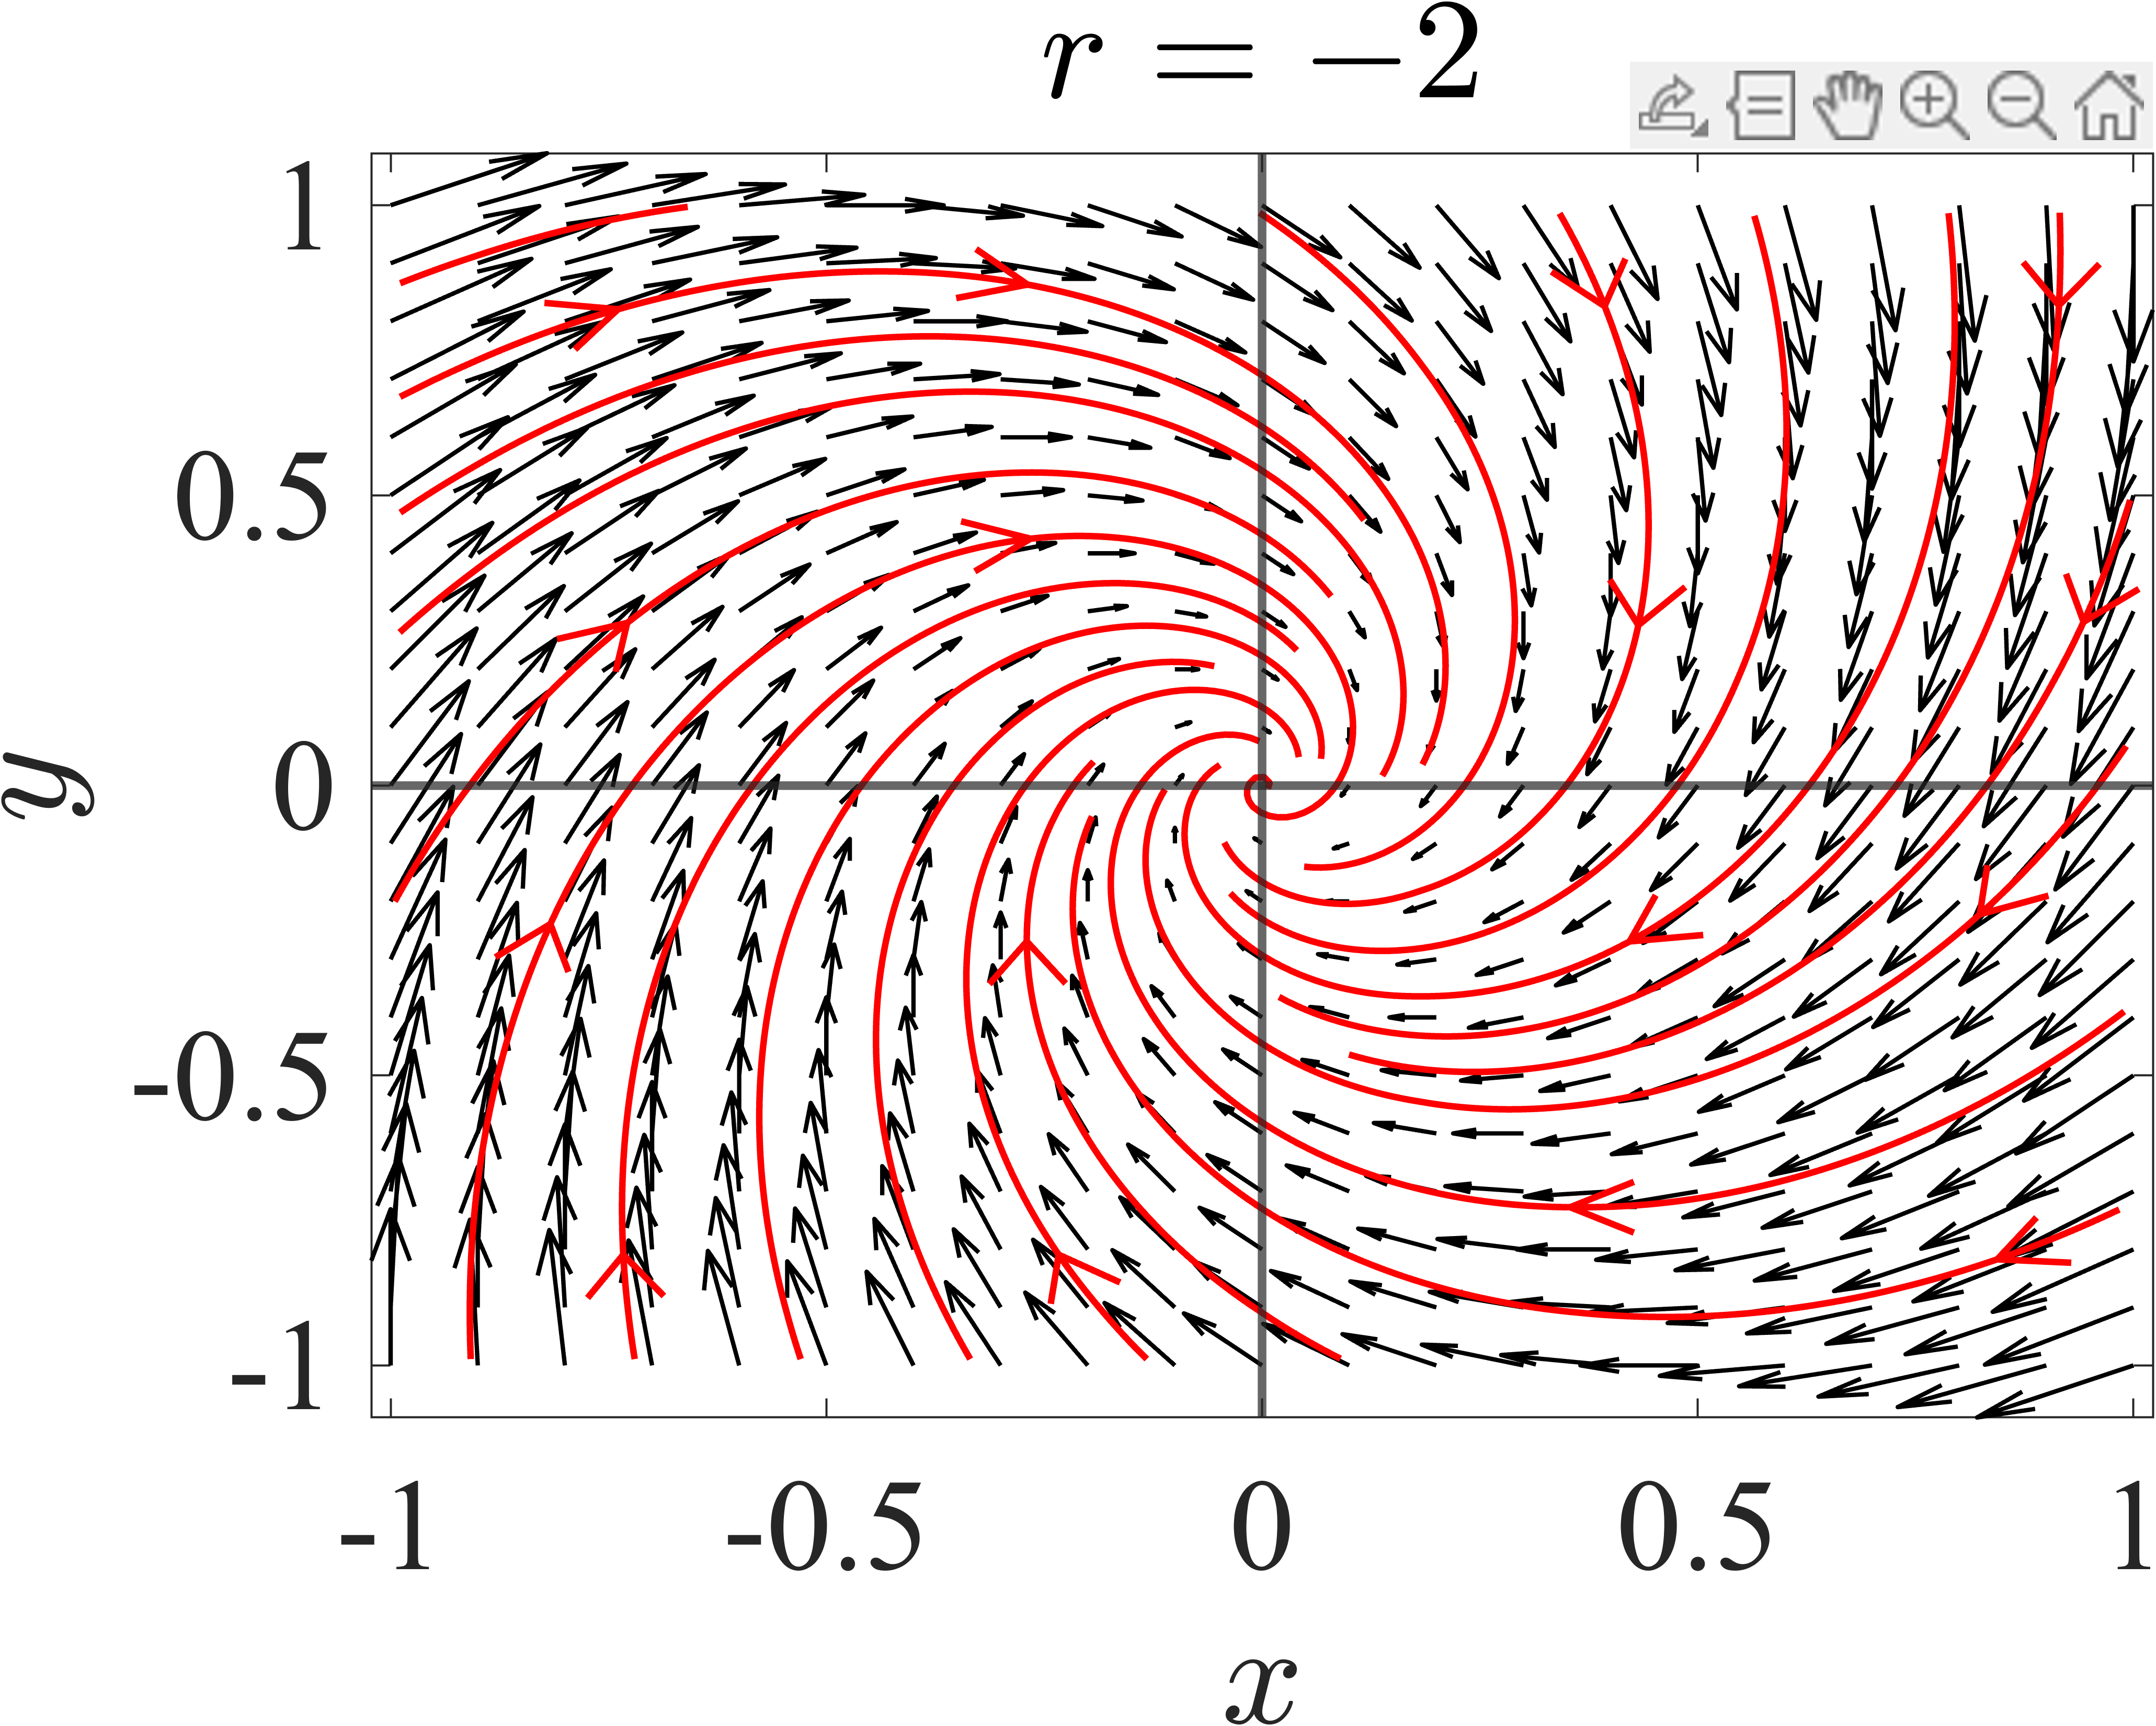
\includegraphics[width=7cm]{phase_portrait_r_-2}
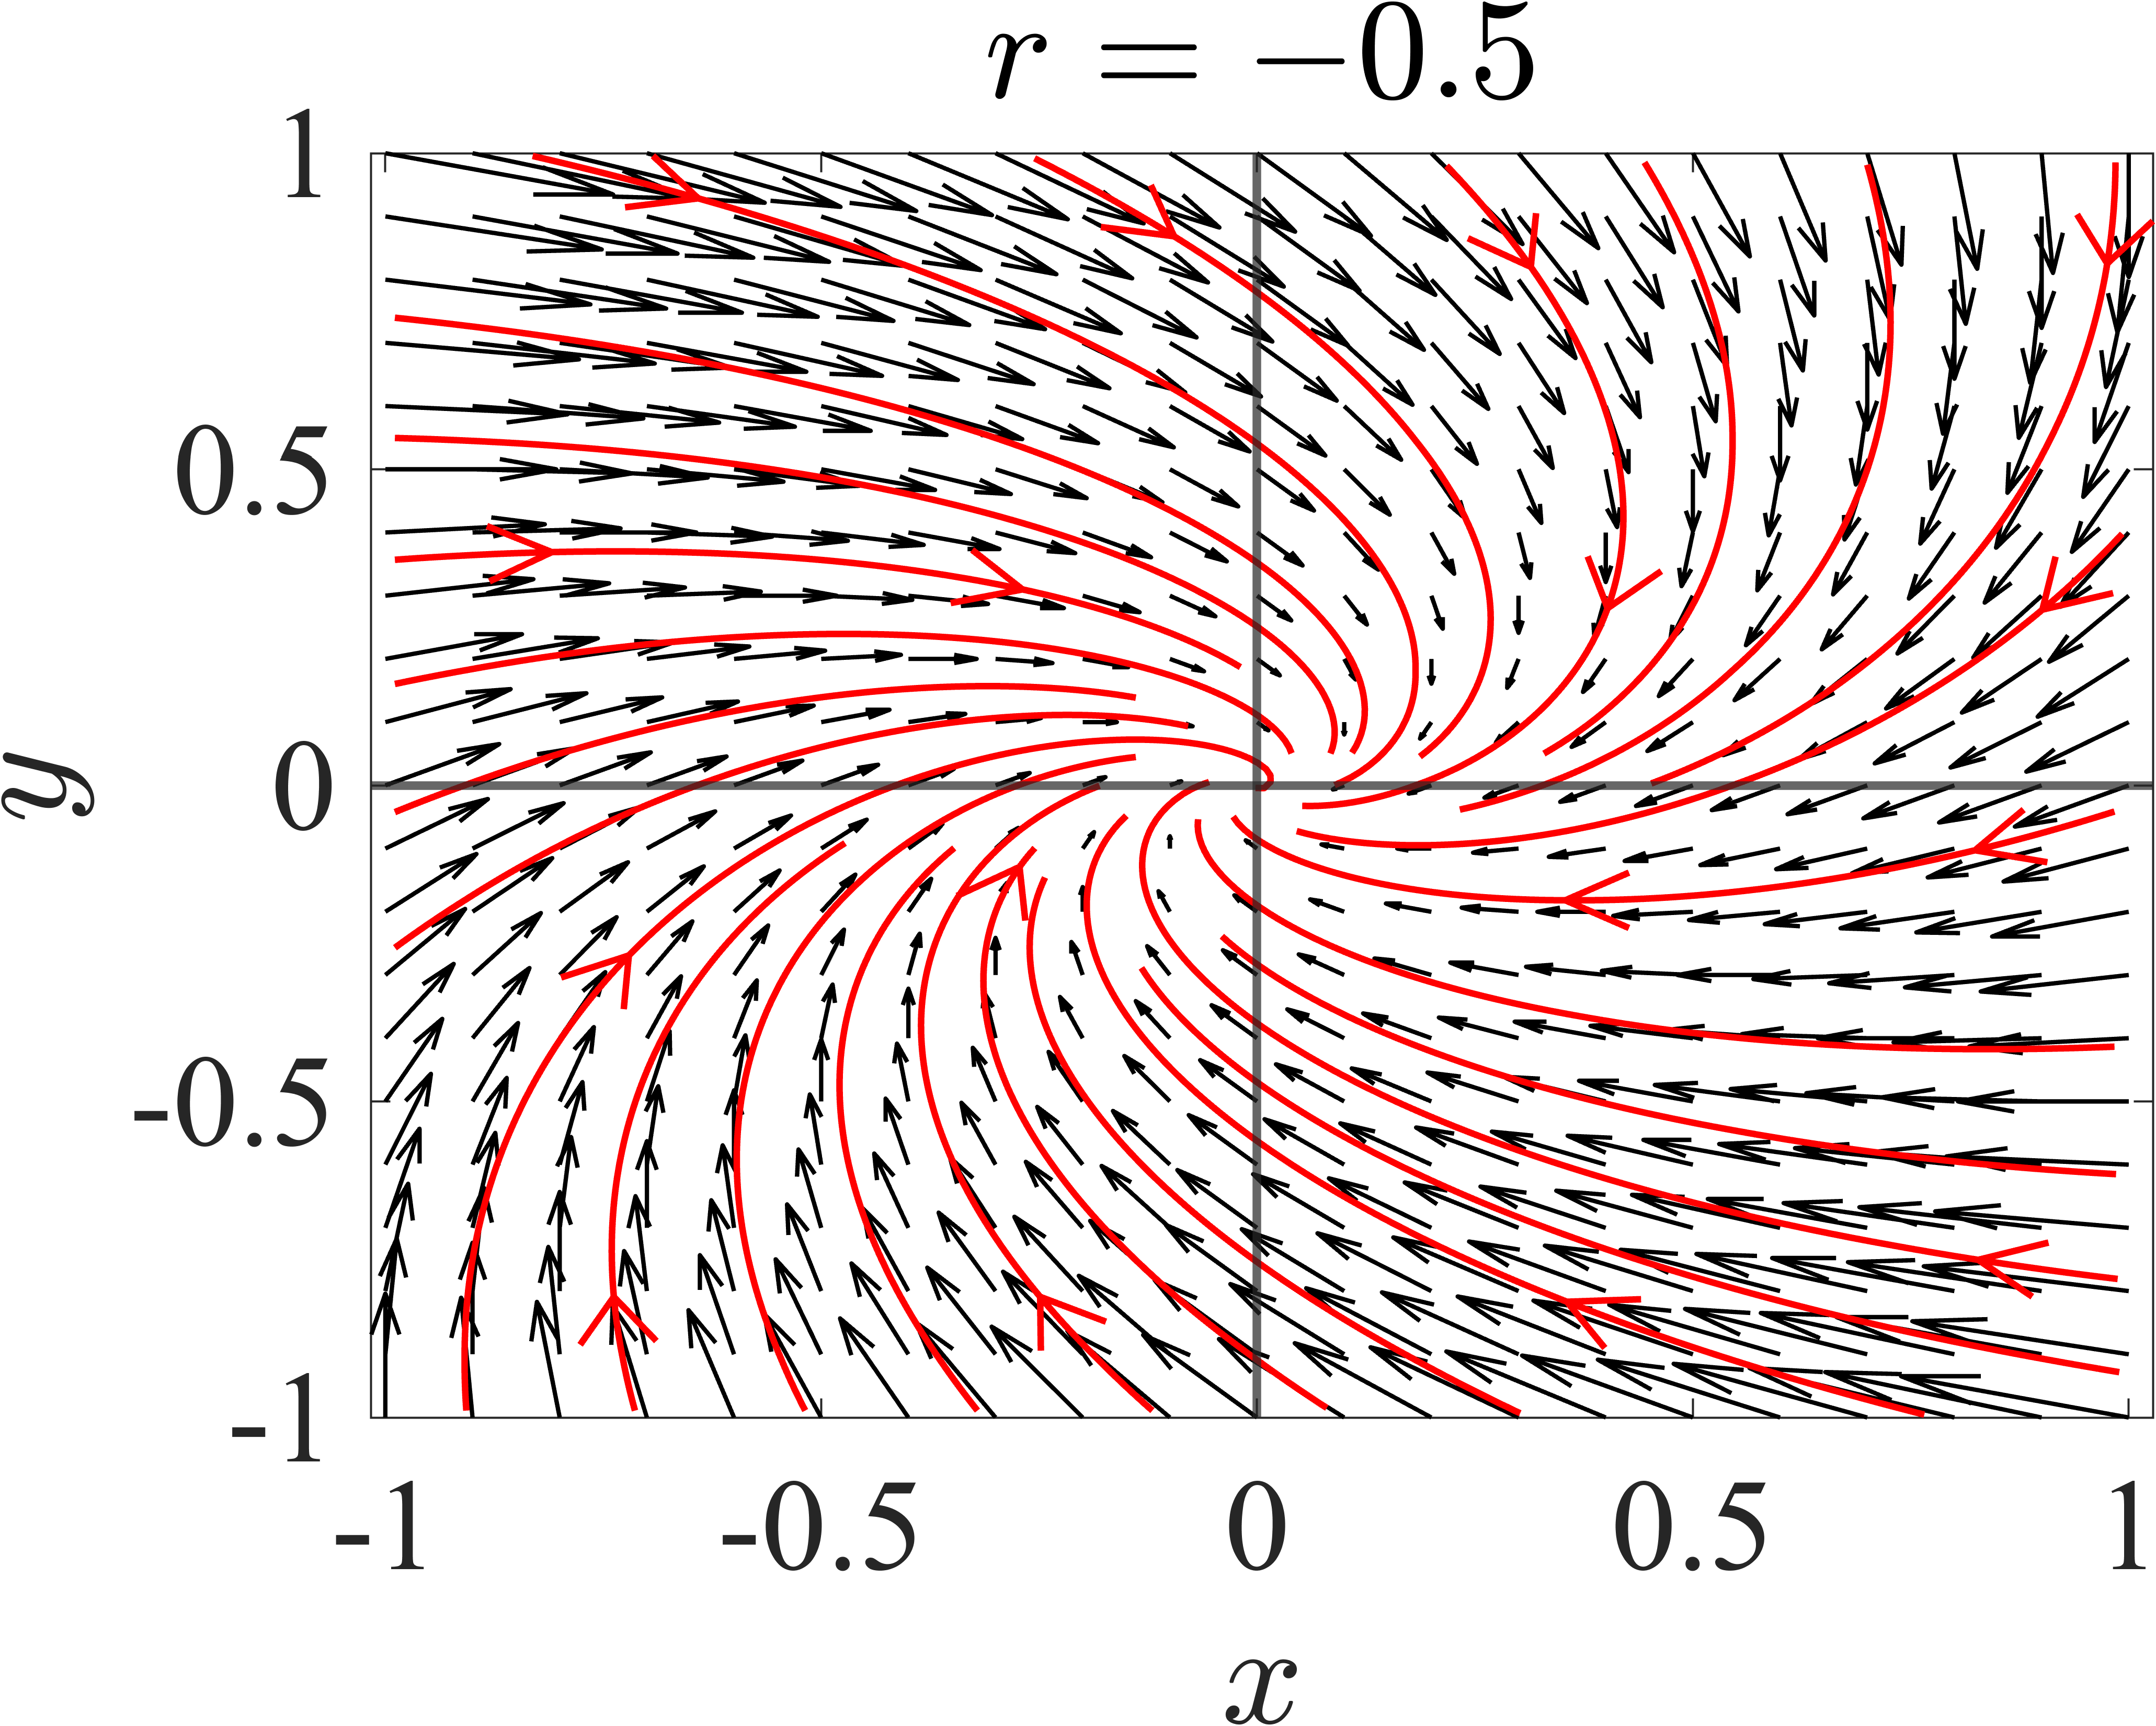
\includegraphics[width=7cm]{phase_portrait_r_-0_5}
\caption{Phase Portraits for $r < 0$}
\end{figure}

\begin{figure}[h]
\centering
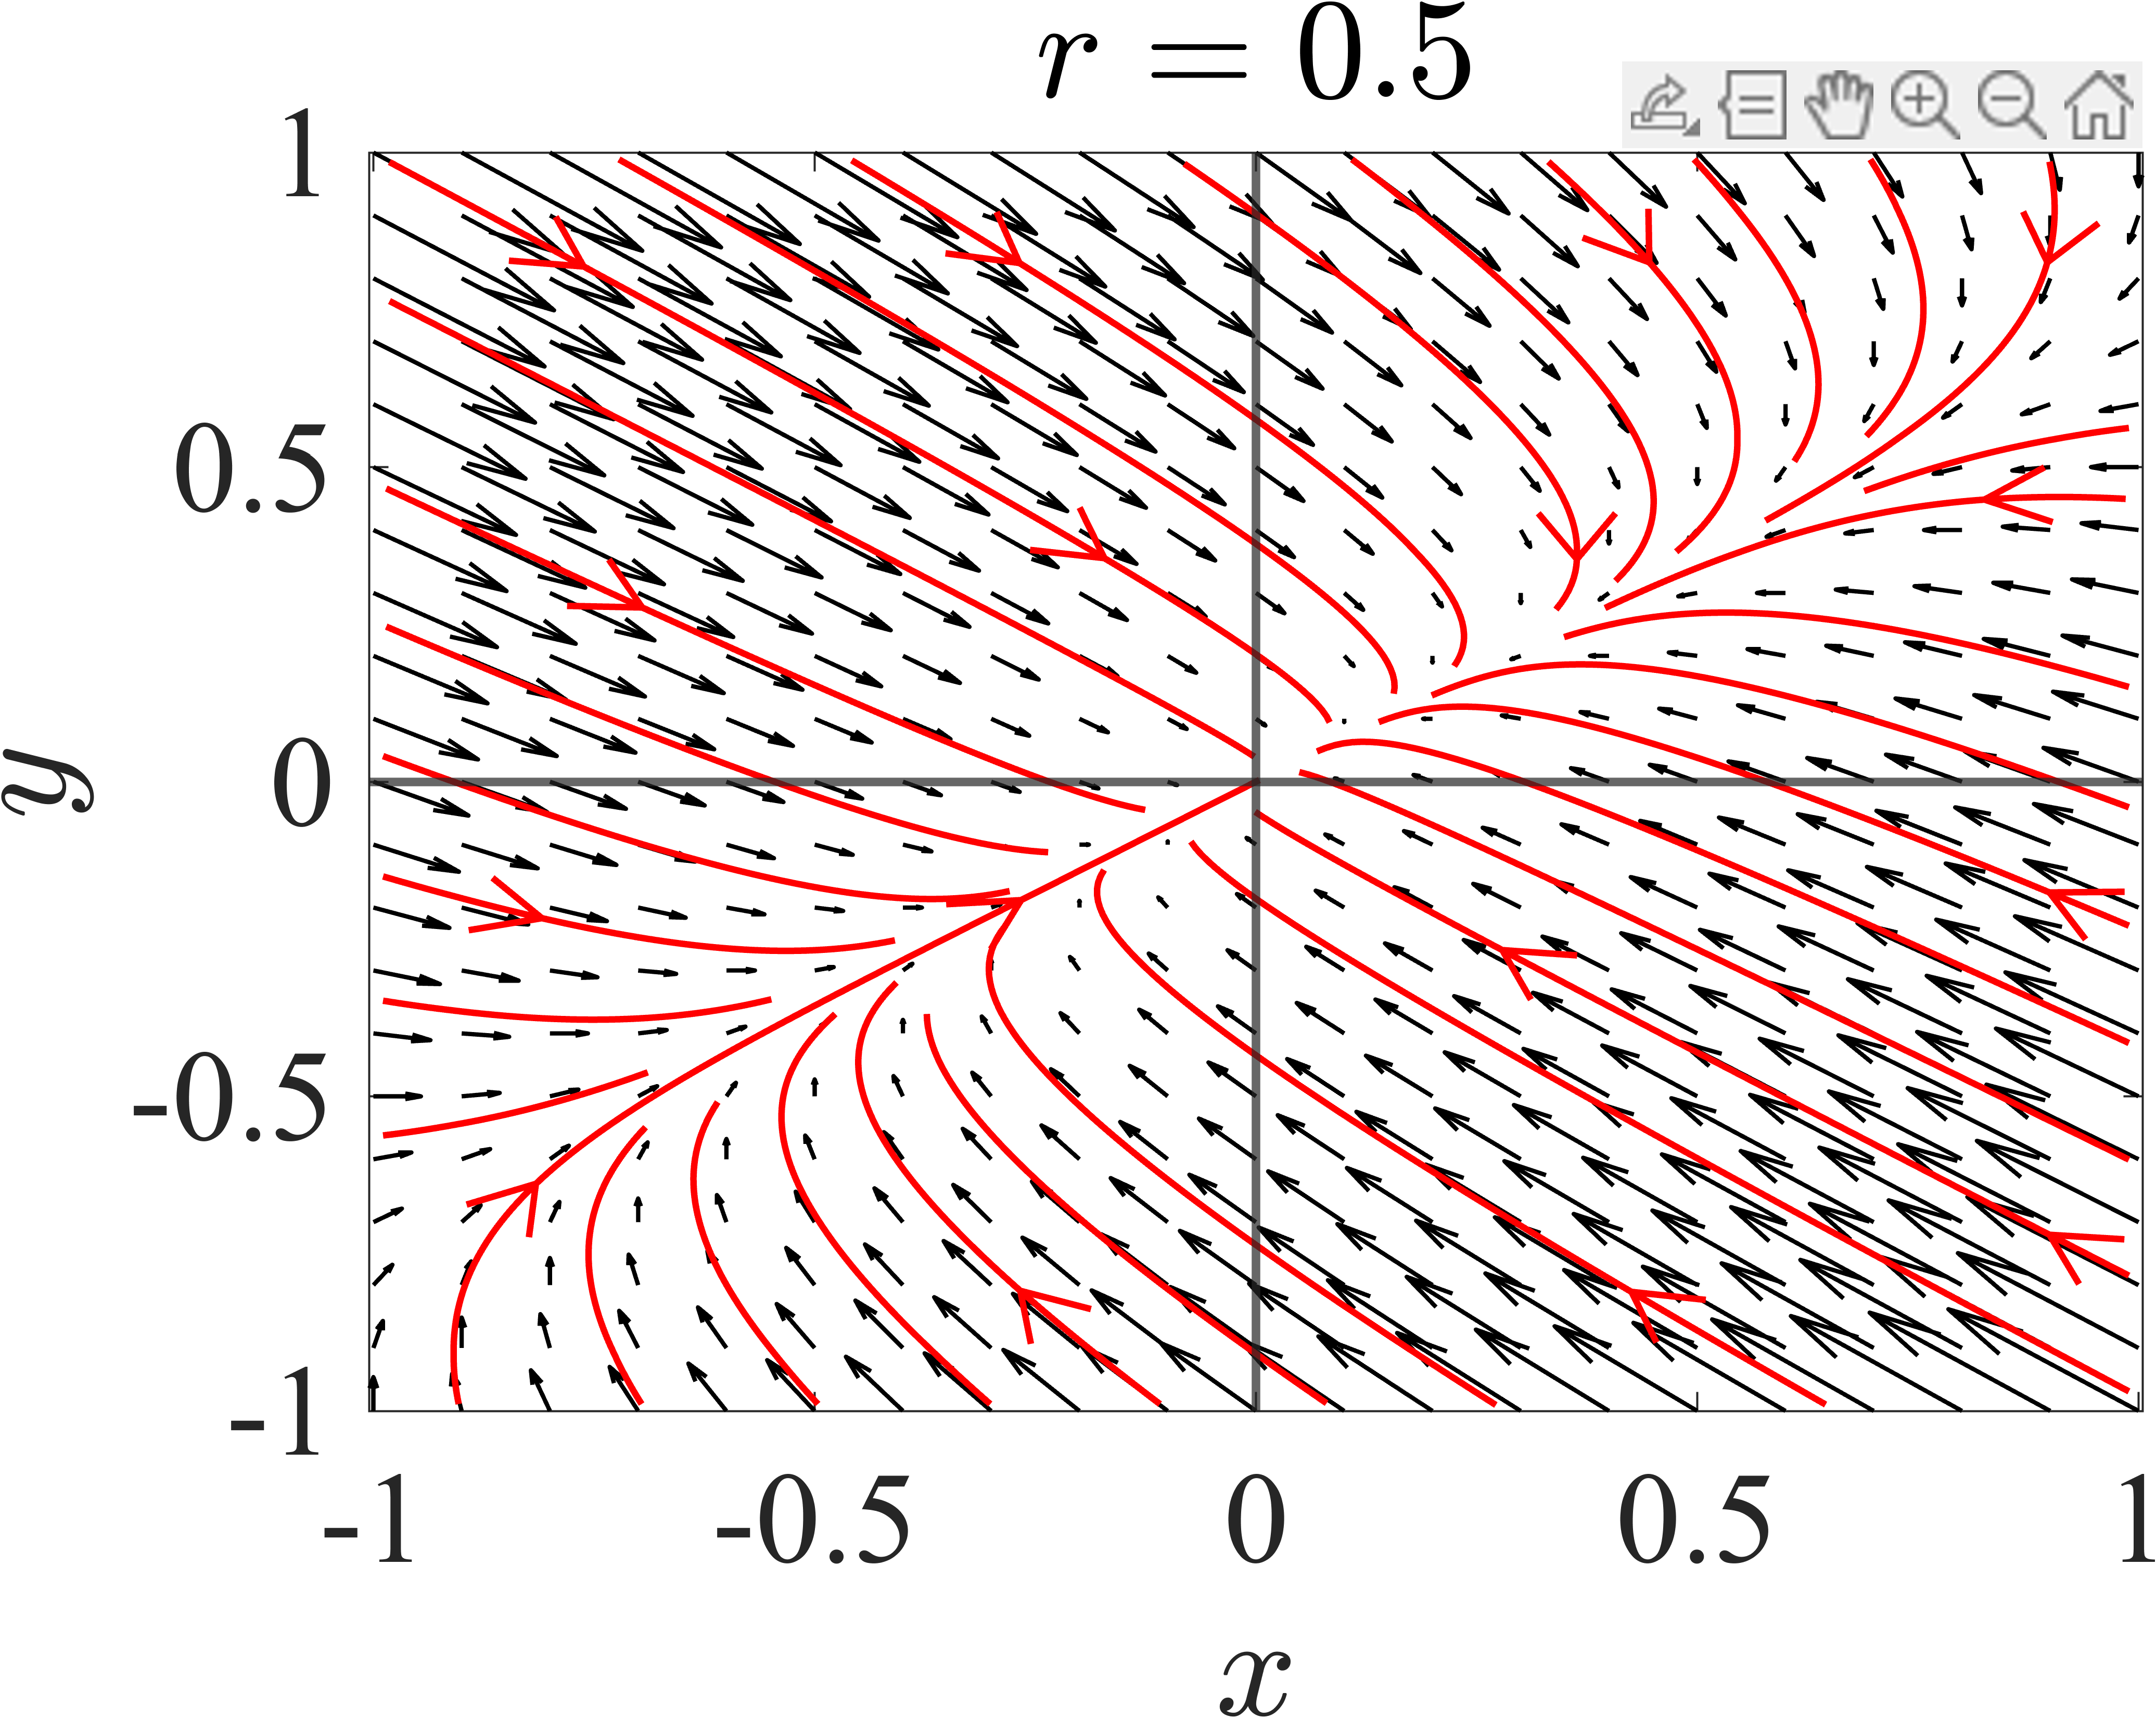
\includegraphics[width=7cm]{phase_portrait_r_0_5}
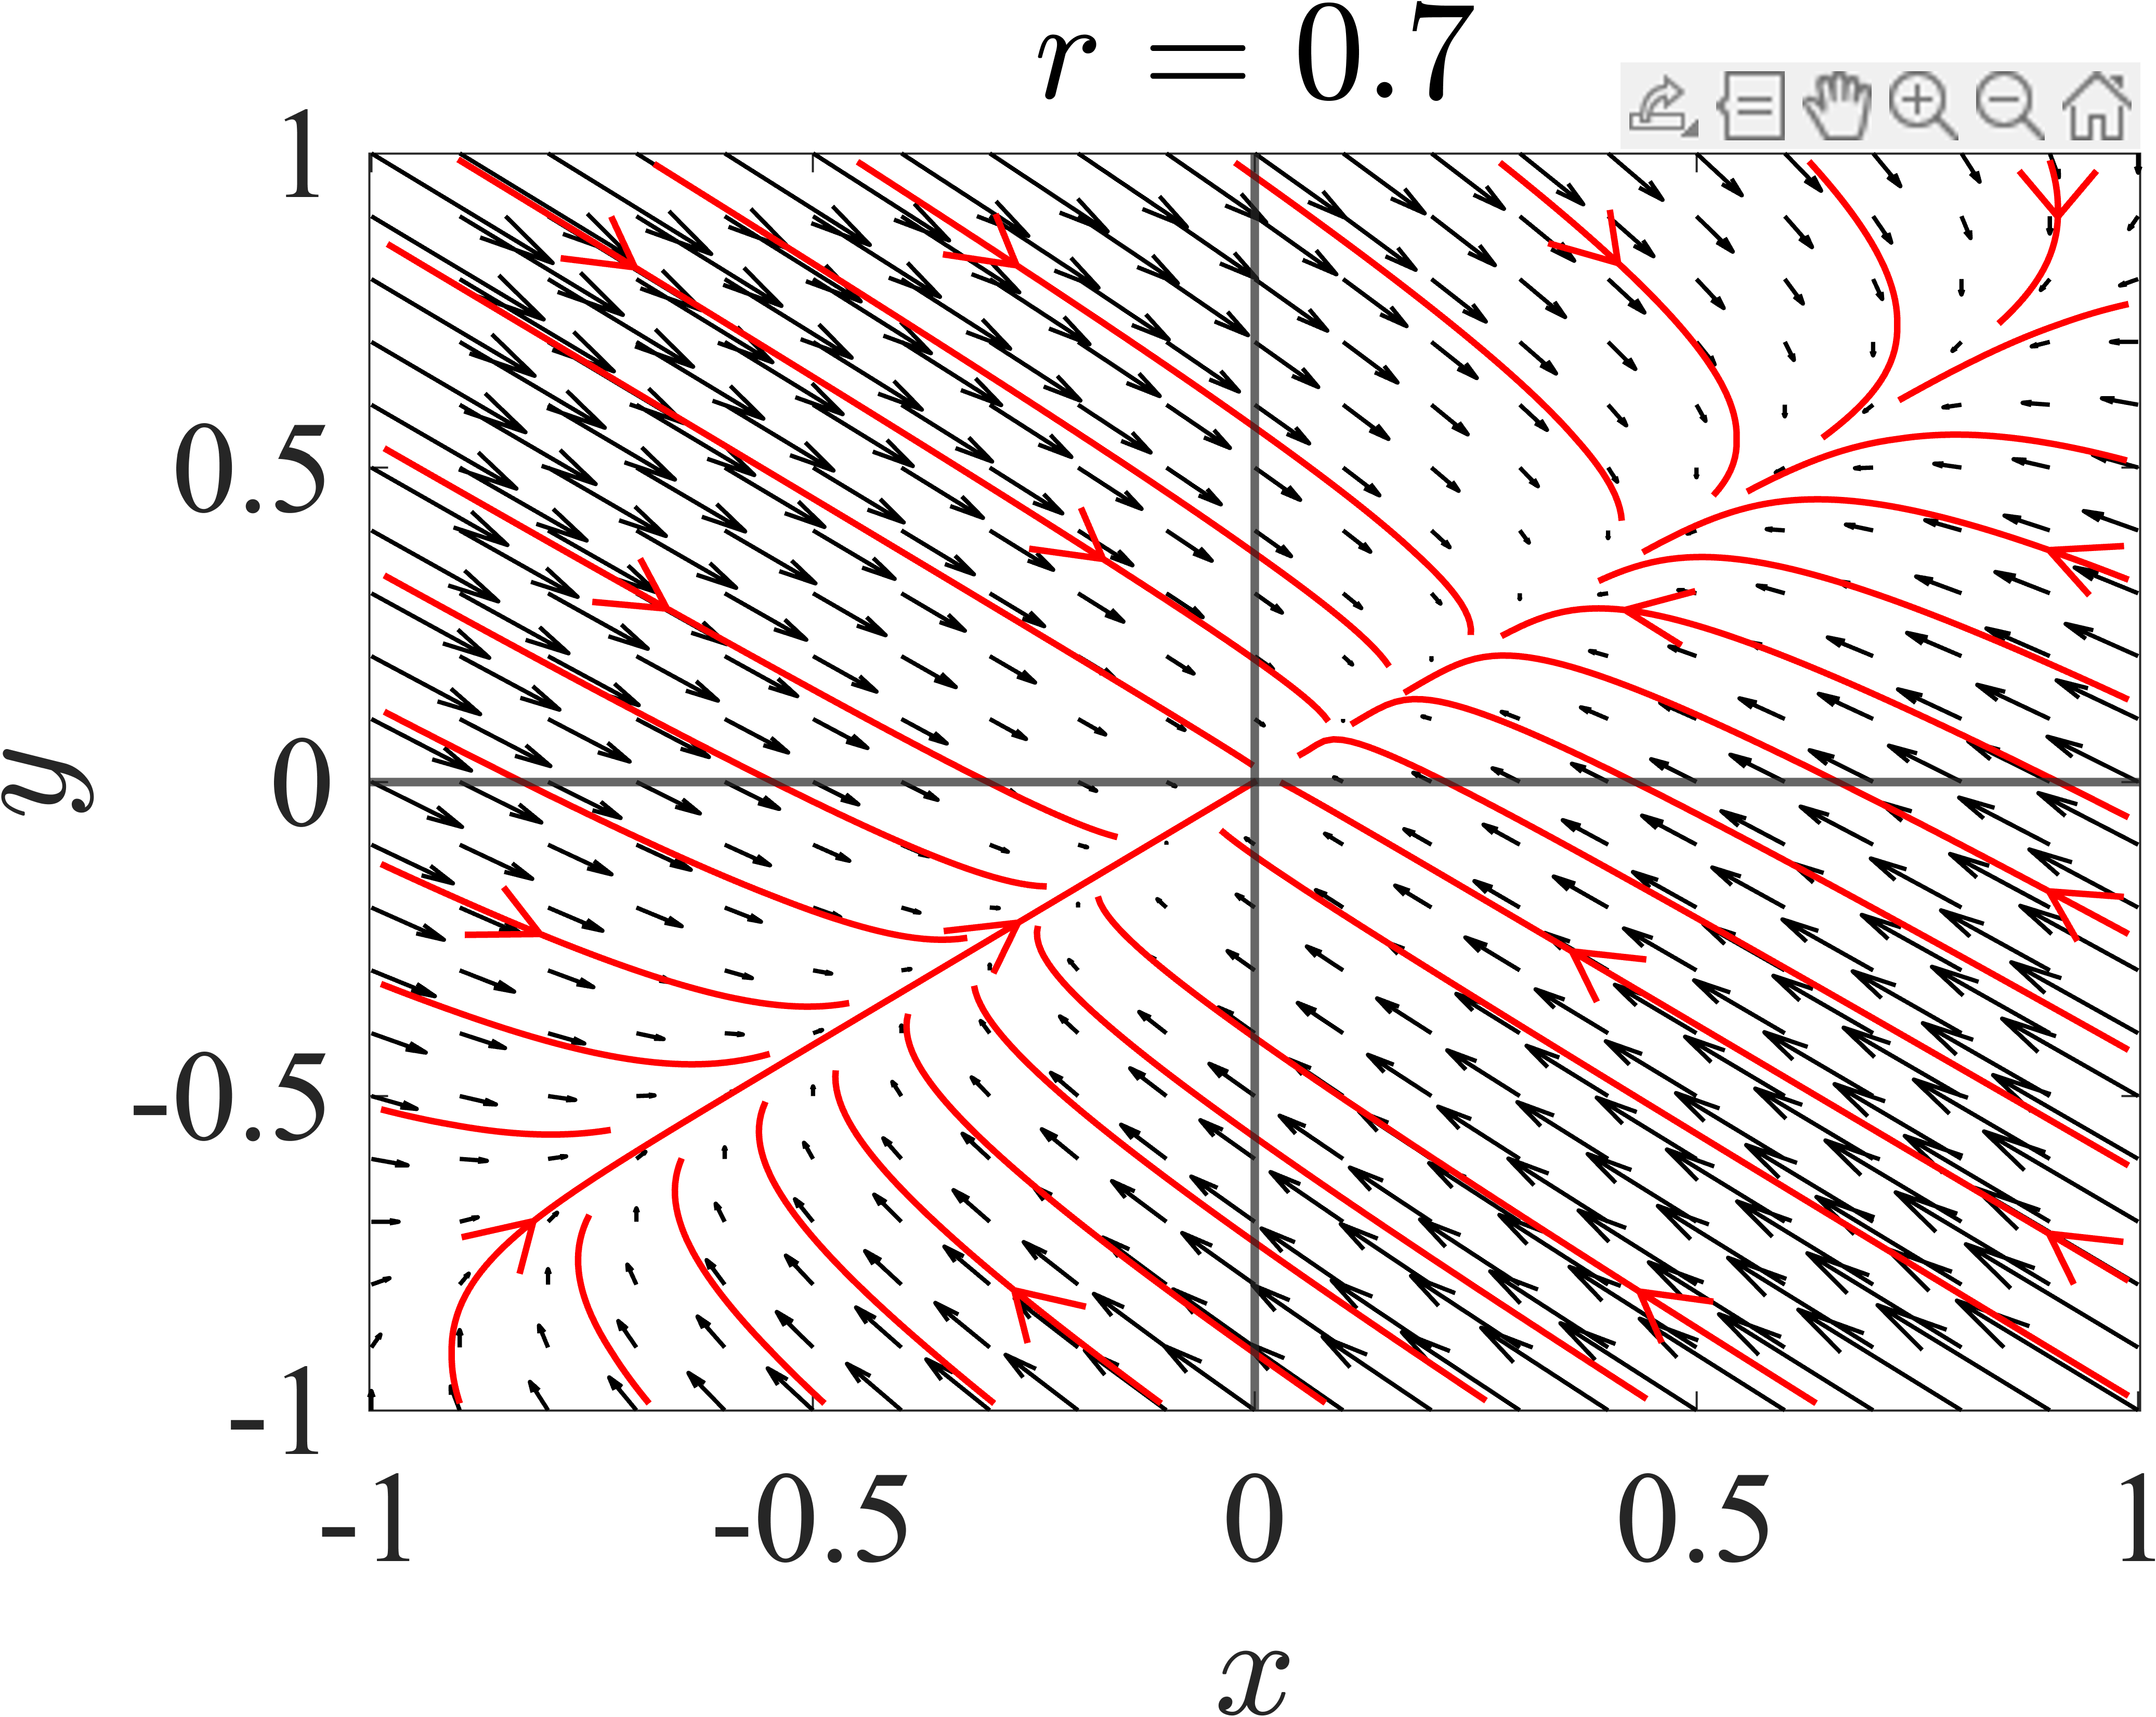
\includegraphics[width=7cm]{phase_portrait_r_0_7}
\caption{Phase Portraits for $0<r<1$}
\end{figure}

\begin{figure}[h]
\centering
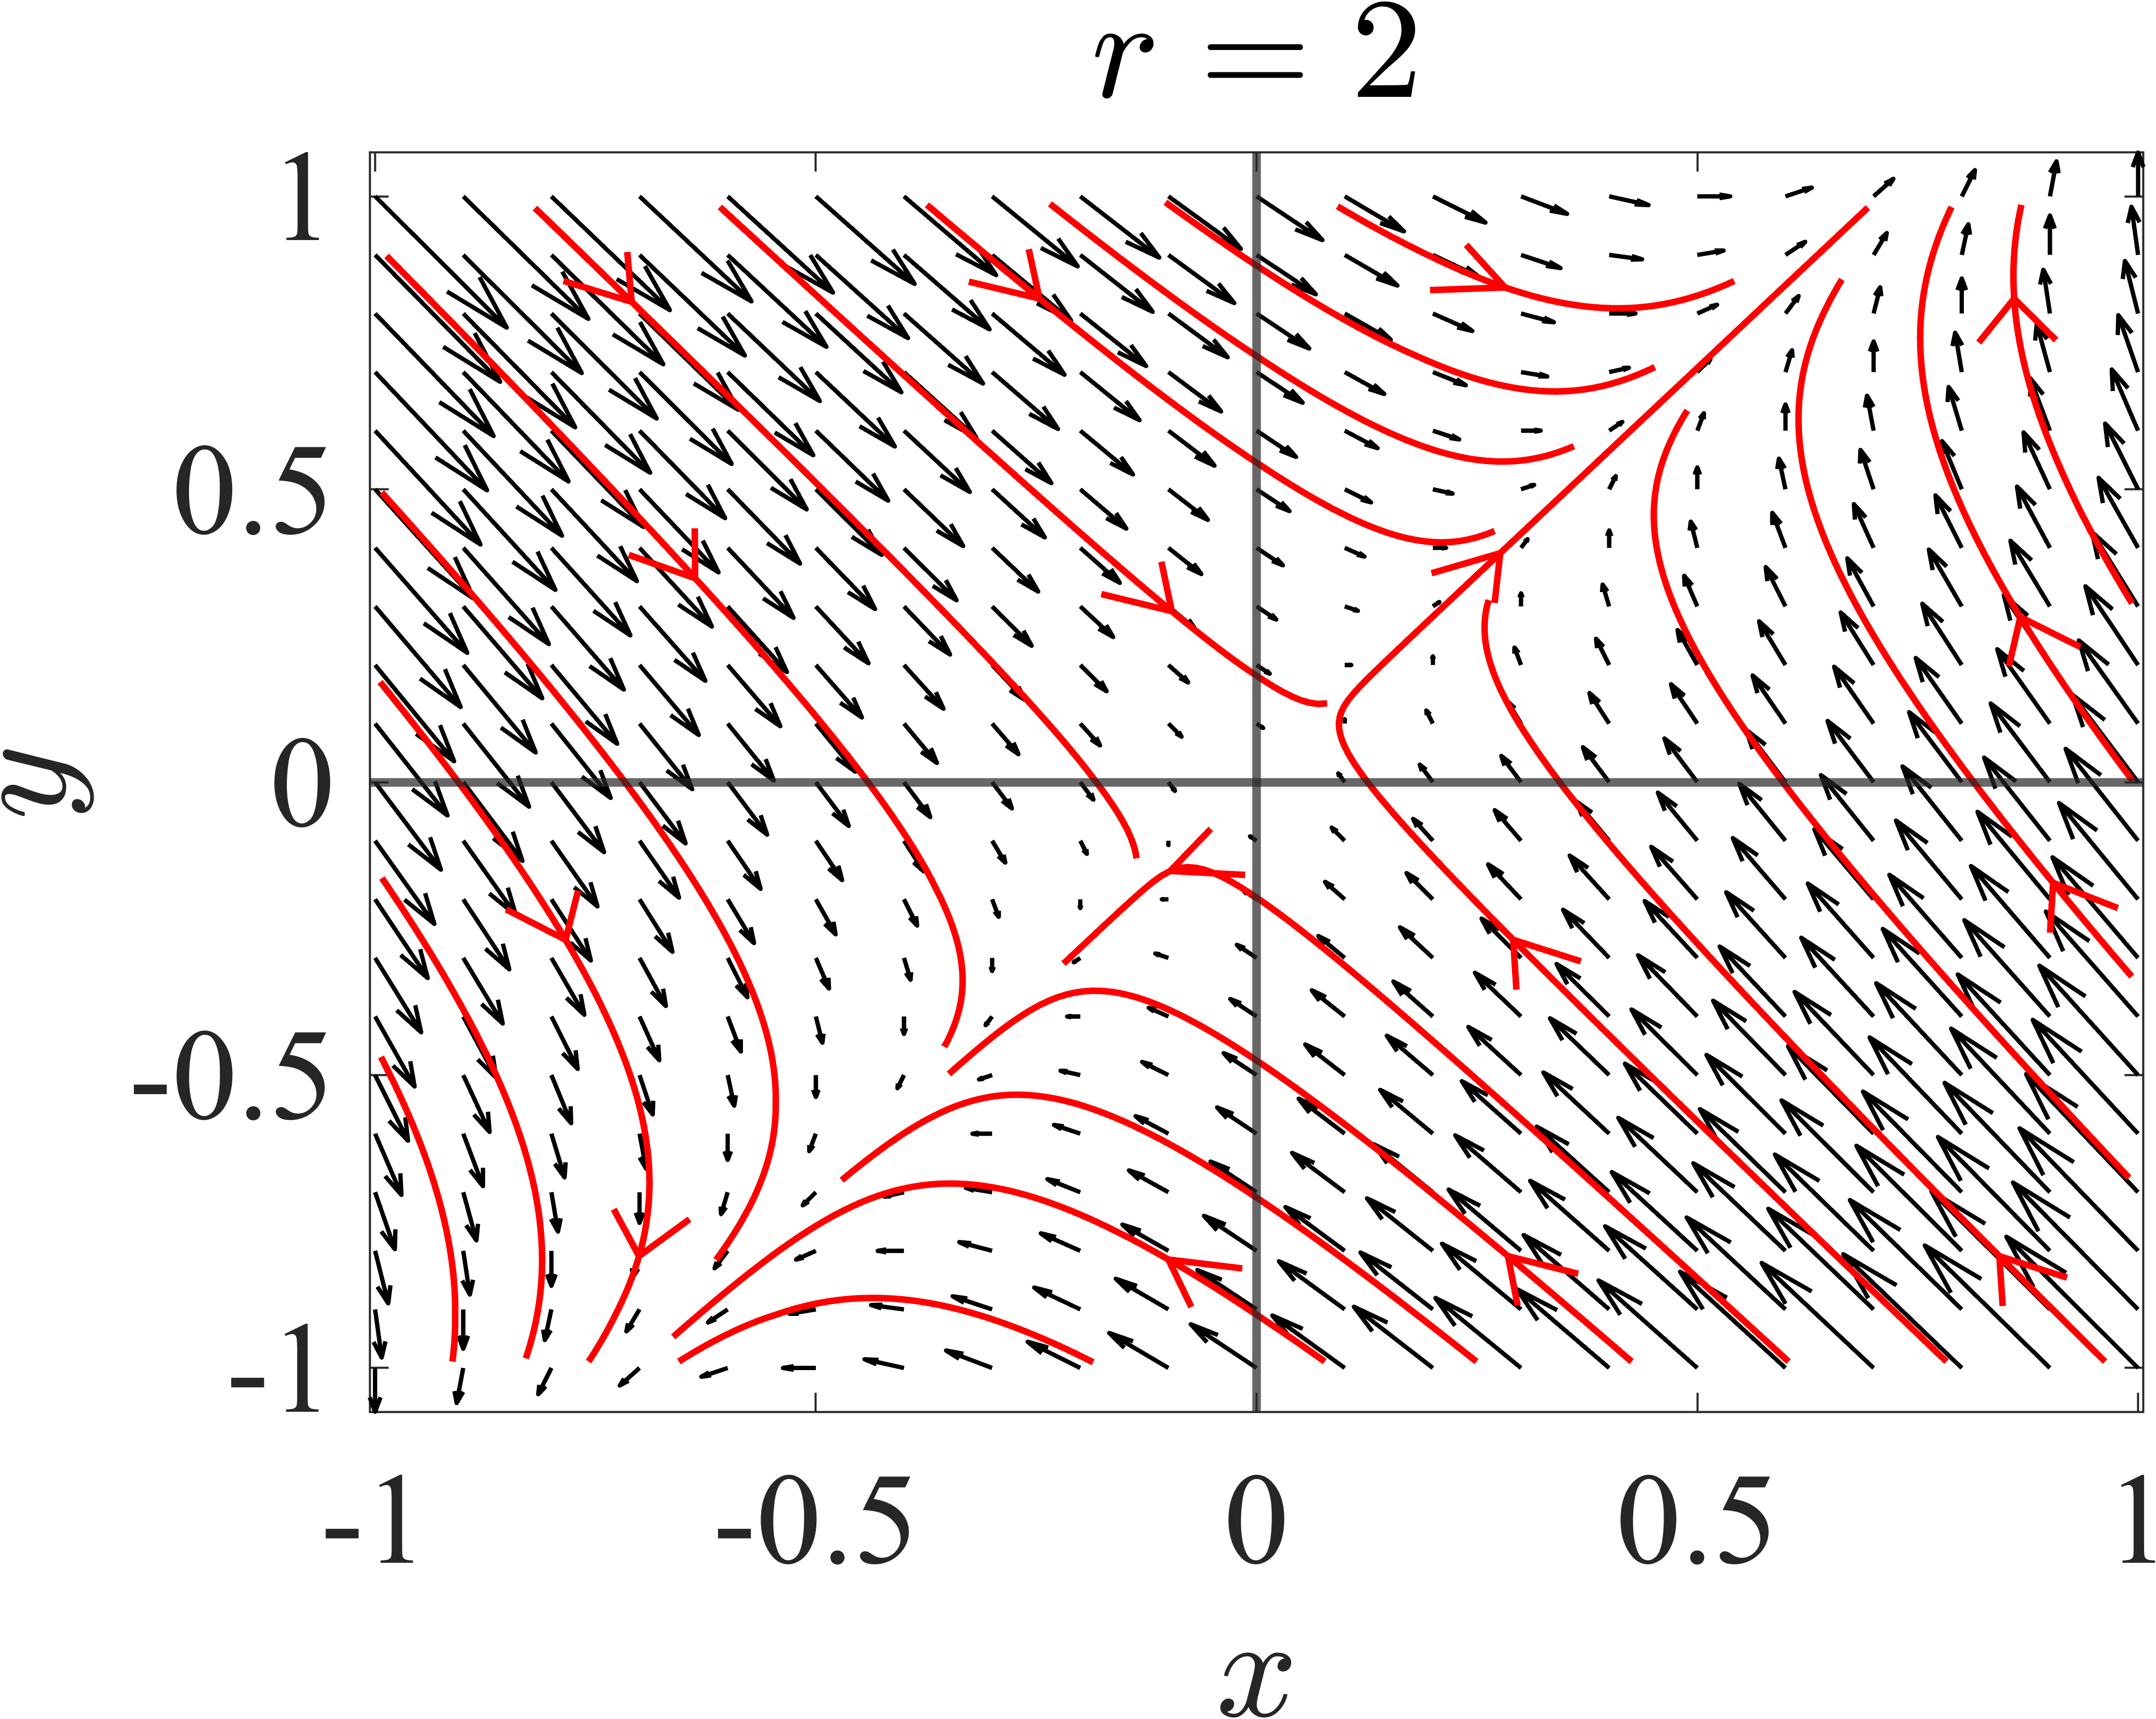
\includegraphics[width=7cm]{phase_portrait_r_2}
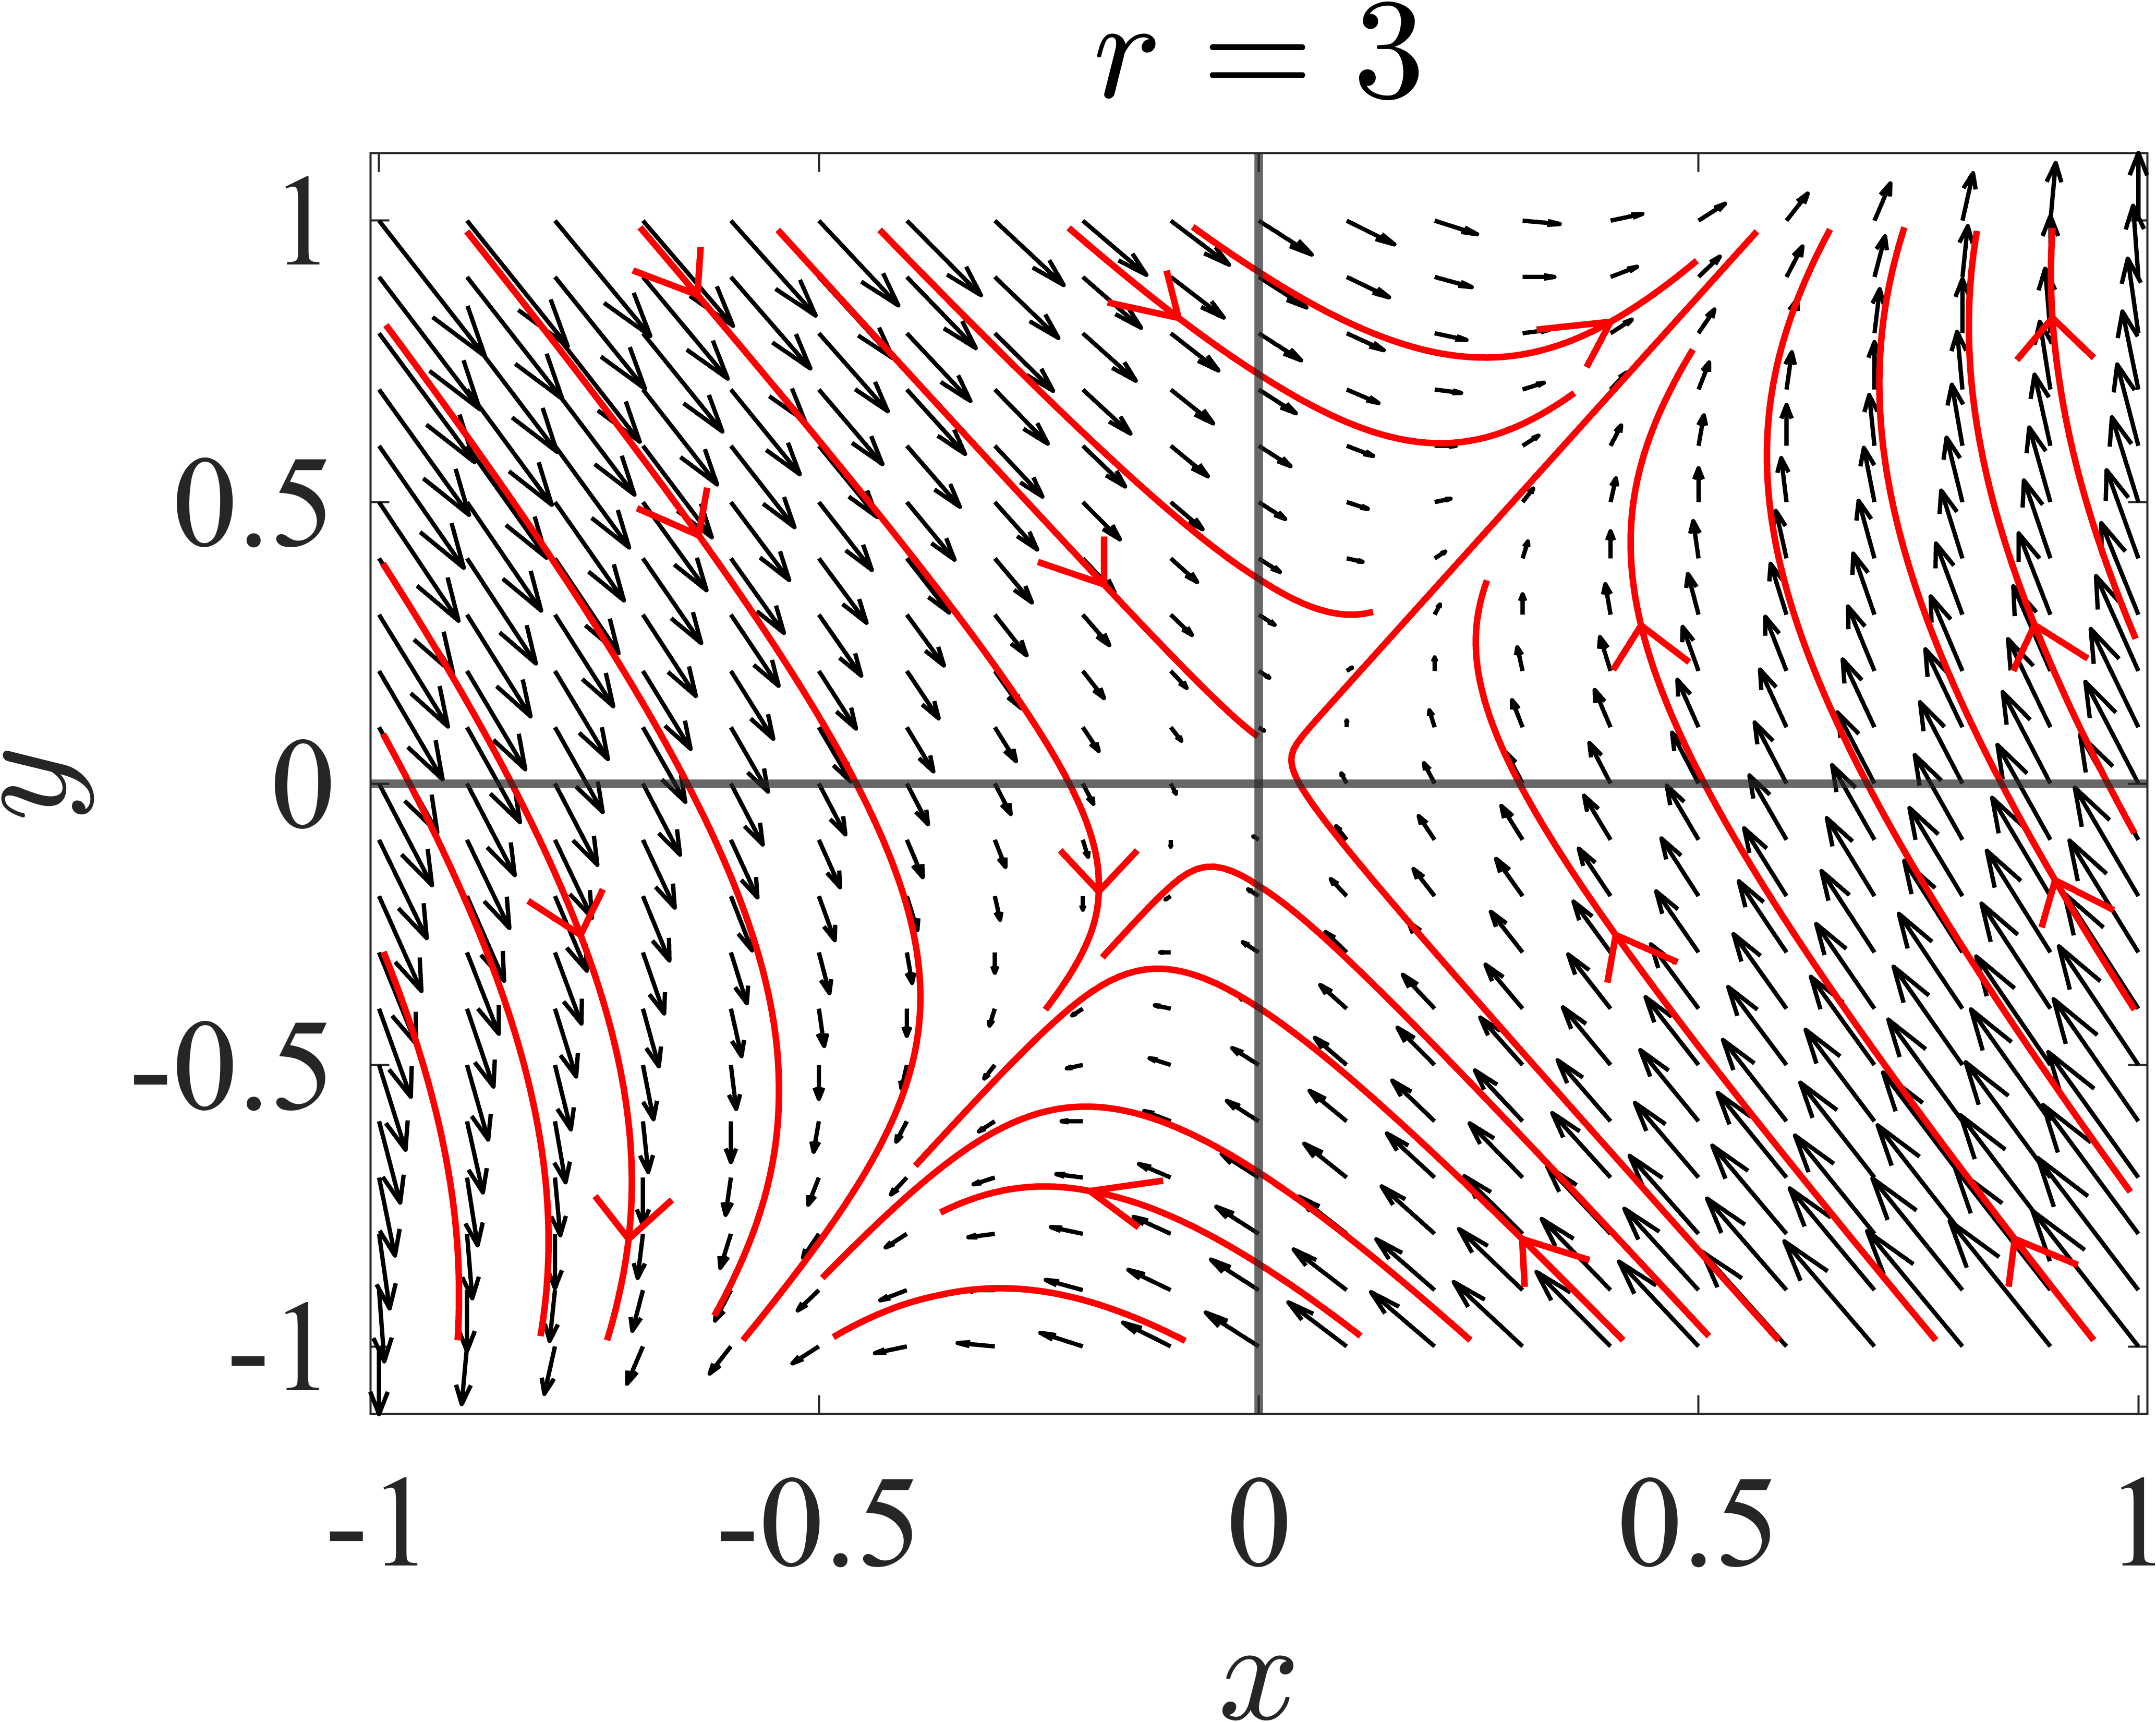
\includegraphics[width=7cm]{phase_portrait_r_3}
\caption{Phase Portraits for $r>1$}
\end{figure}

\begin{figure}[h]
\centering
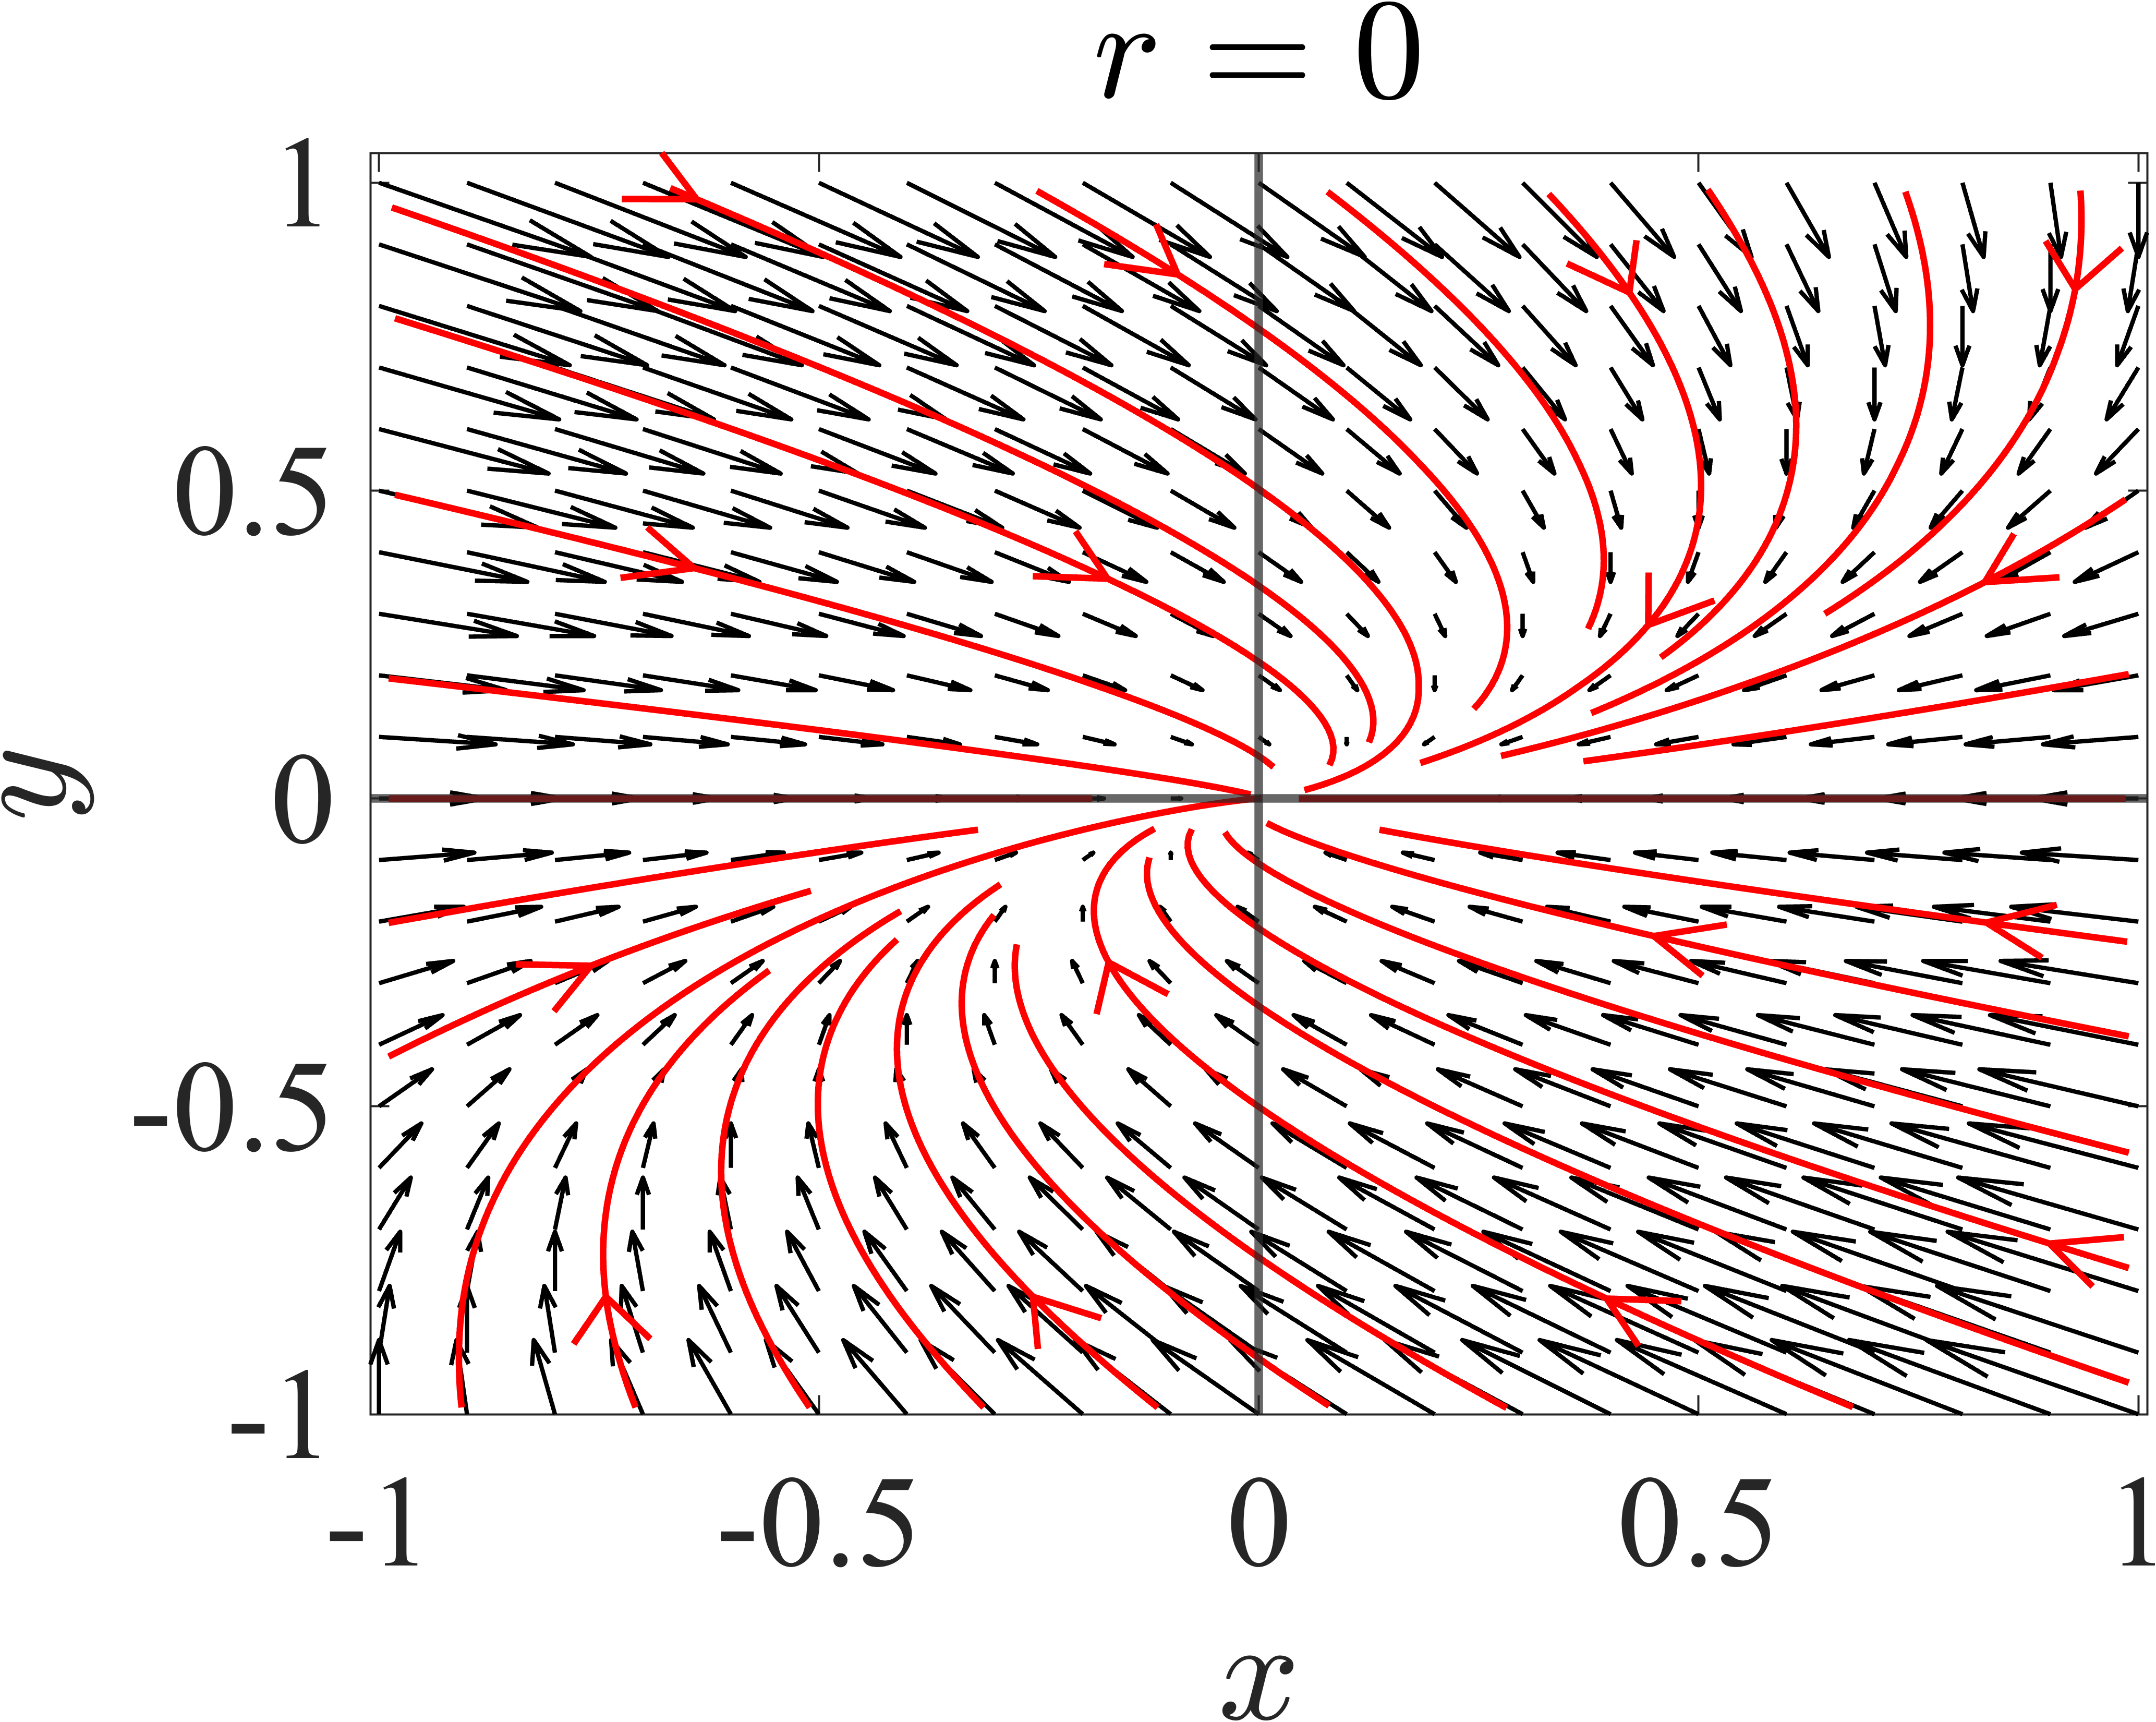
\includegraphics[width=7cm]{phase_portrait_r_0}
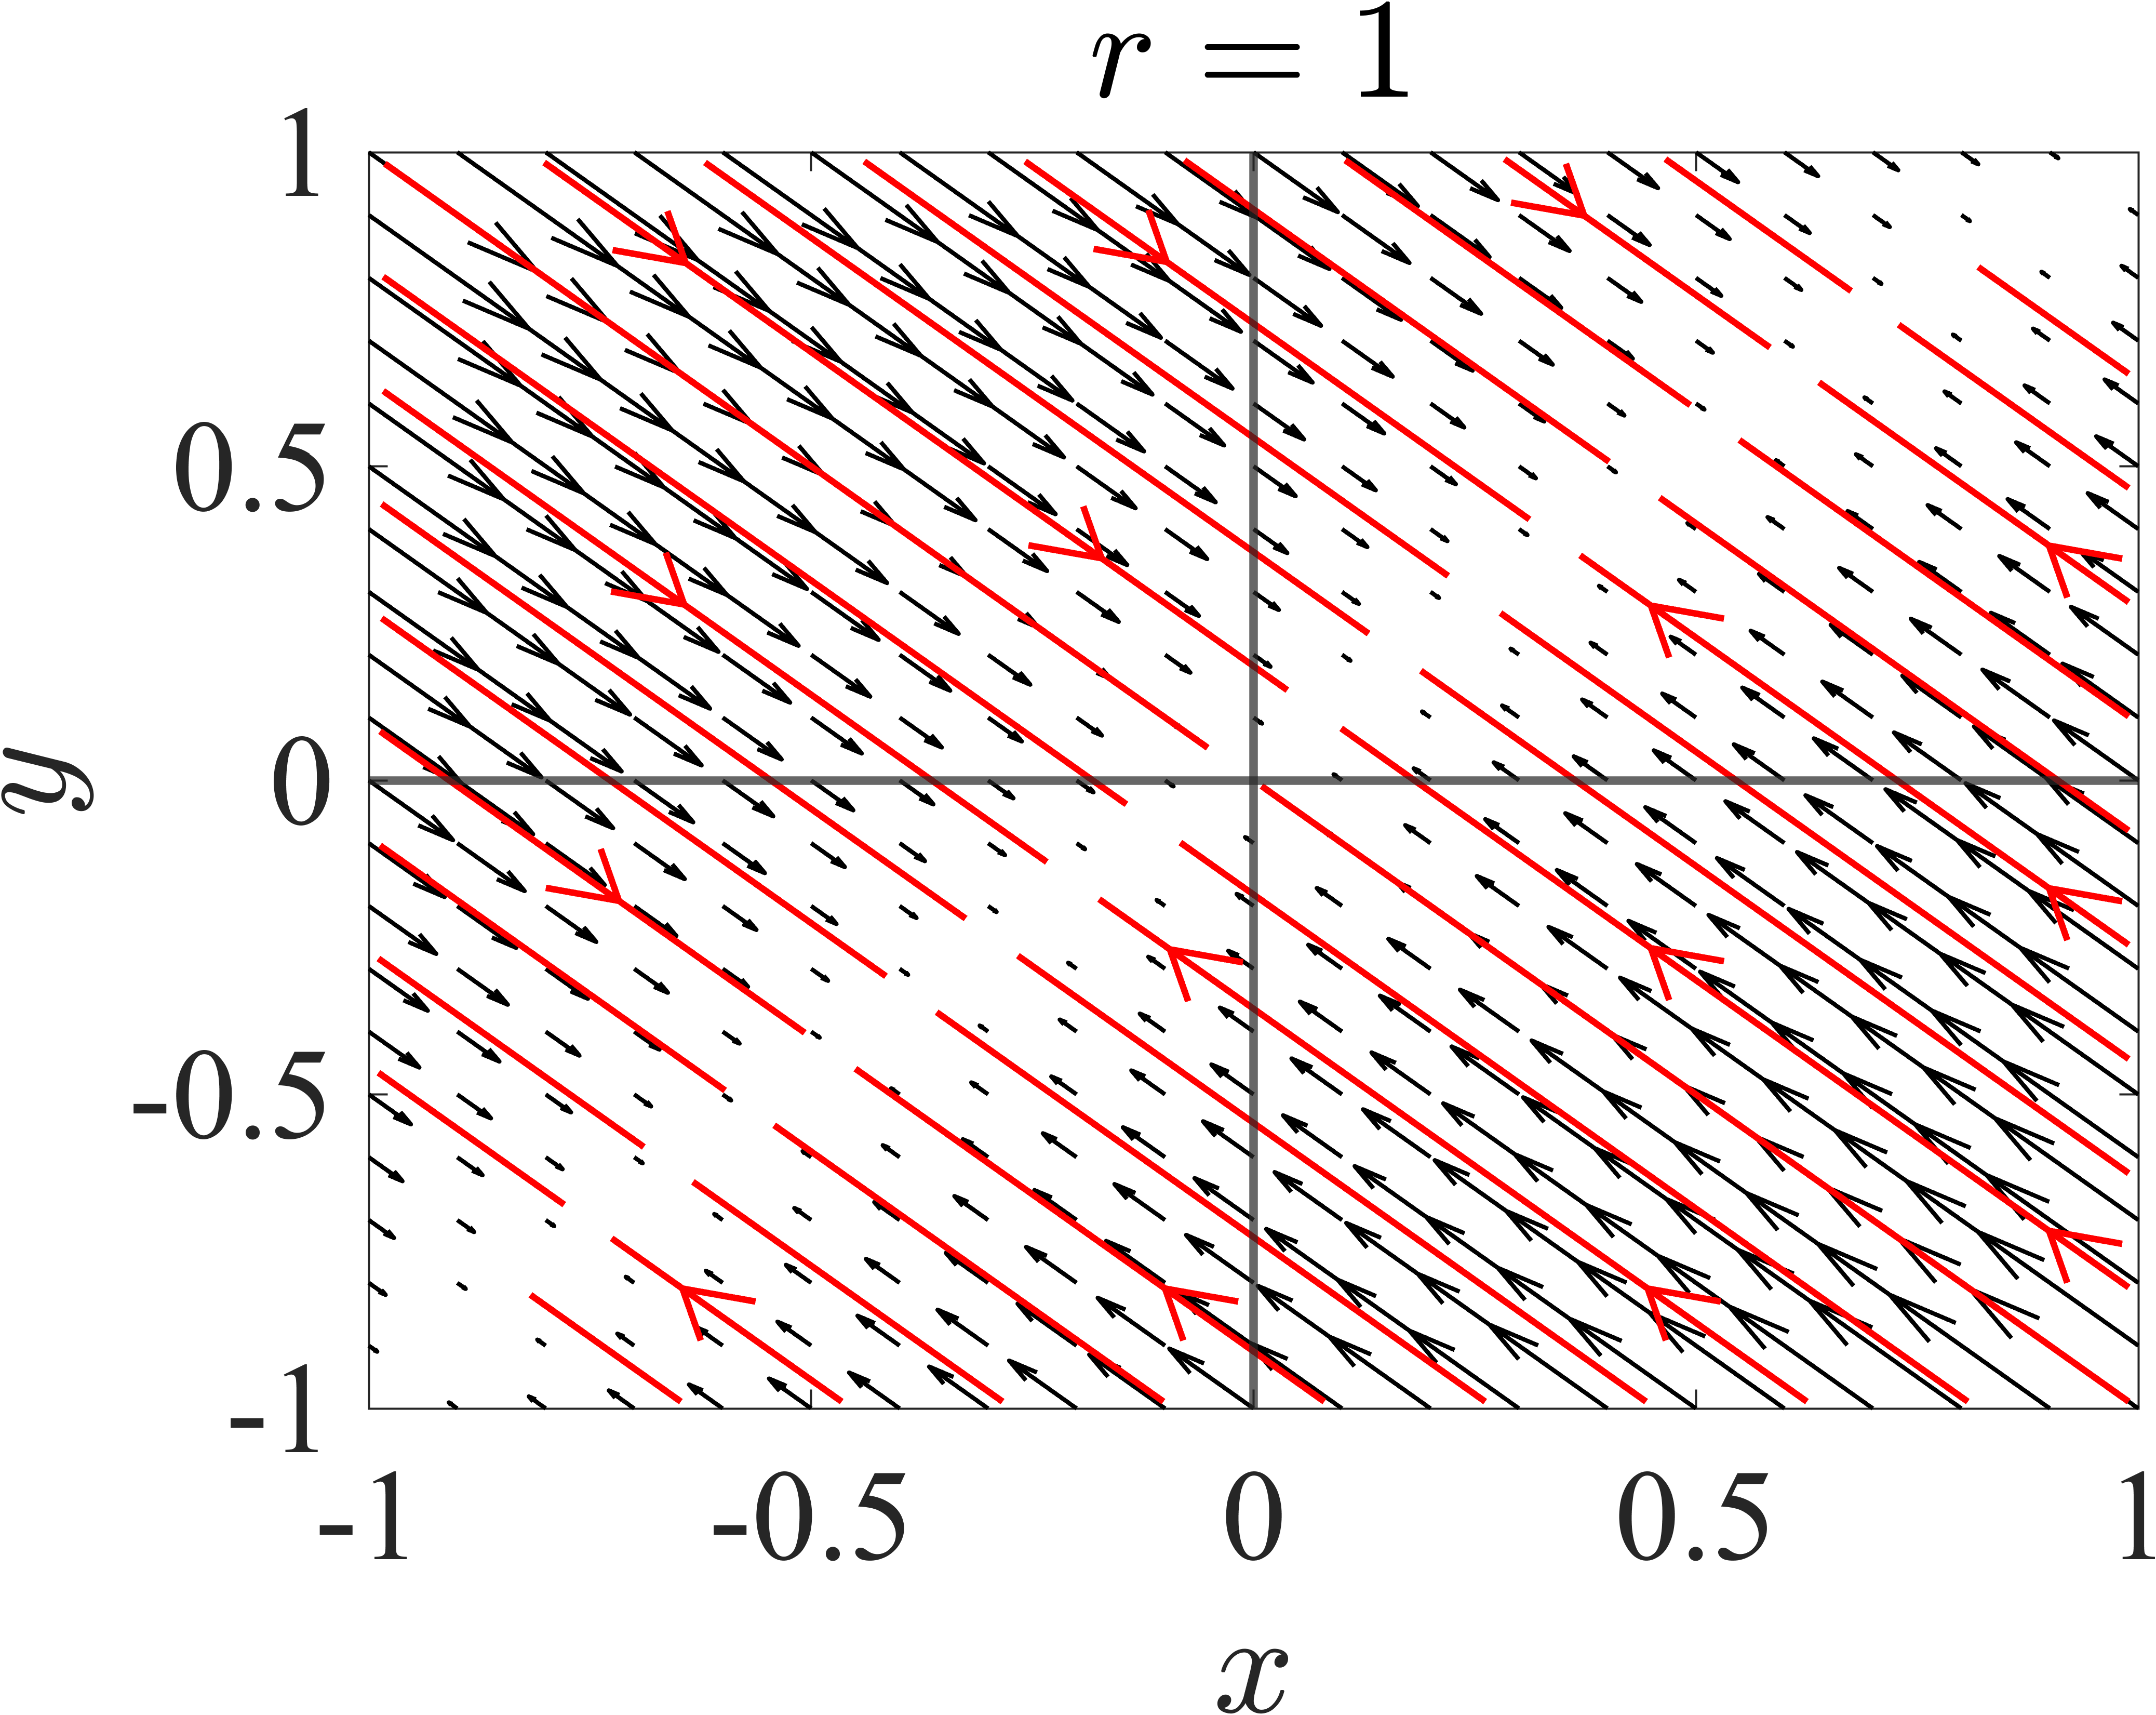
\includegraphics[width=7cm]{phase_portrait_r_1}
\caption{Phase Portraits for Marginal Cases}
\end{figure}


\end{document}
